\newpage
\question
The table below shows the monthly rent for nine apartments and the distance of these apartments from
the city centre.
\begin{table}[H]
    \centering
 \begin{tabular}{|l|l|l|l|l|l|l|l|l|l|}
\hline Distance from the city centre $(\mathrm{km})$ & \cellcolor{gray!25}0.8 & \cellcolor{gray!25}1.5 & \cellcolor{gray!25}2.7 & \cellcolor{gray!25}3.6 & 2.0 & 4.3 & 2.3 & 3.0 & 1.0 \\
\hline Monthly rent (\$) & \cellcolor{gray!25}570 & \cellcolor{gray!25}470 & \cellcolor{gray!25}420 & \cellcolor{gray!25}300 & 480 & 270 & 390 & 360 & 530 \\
\hline
\end{tabular}
\end{table}
\begin{center}
        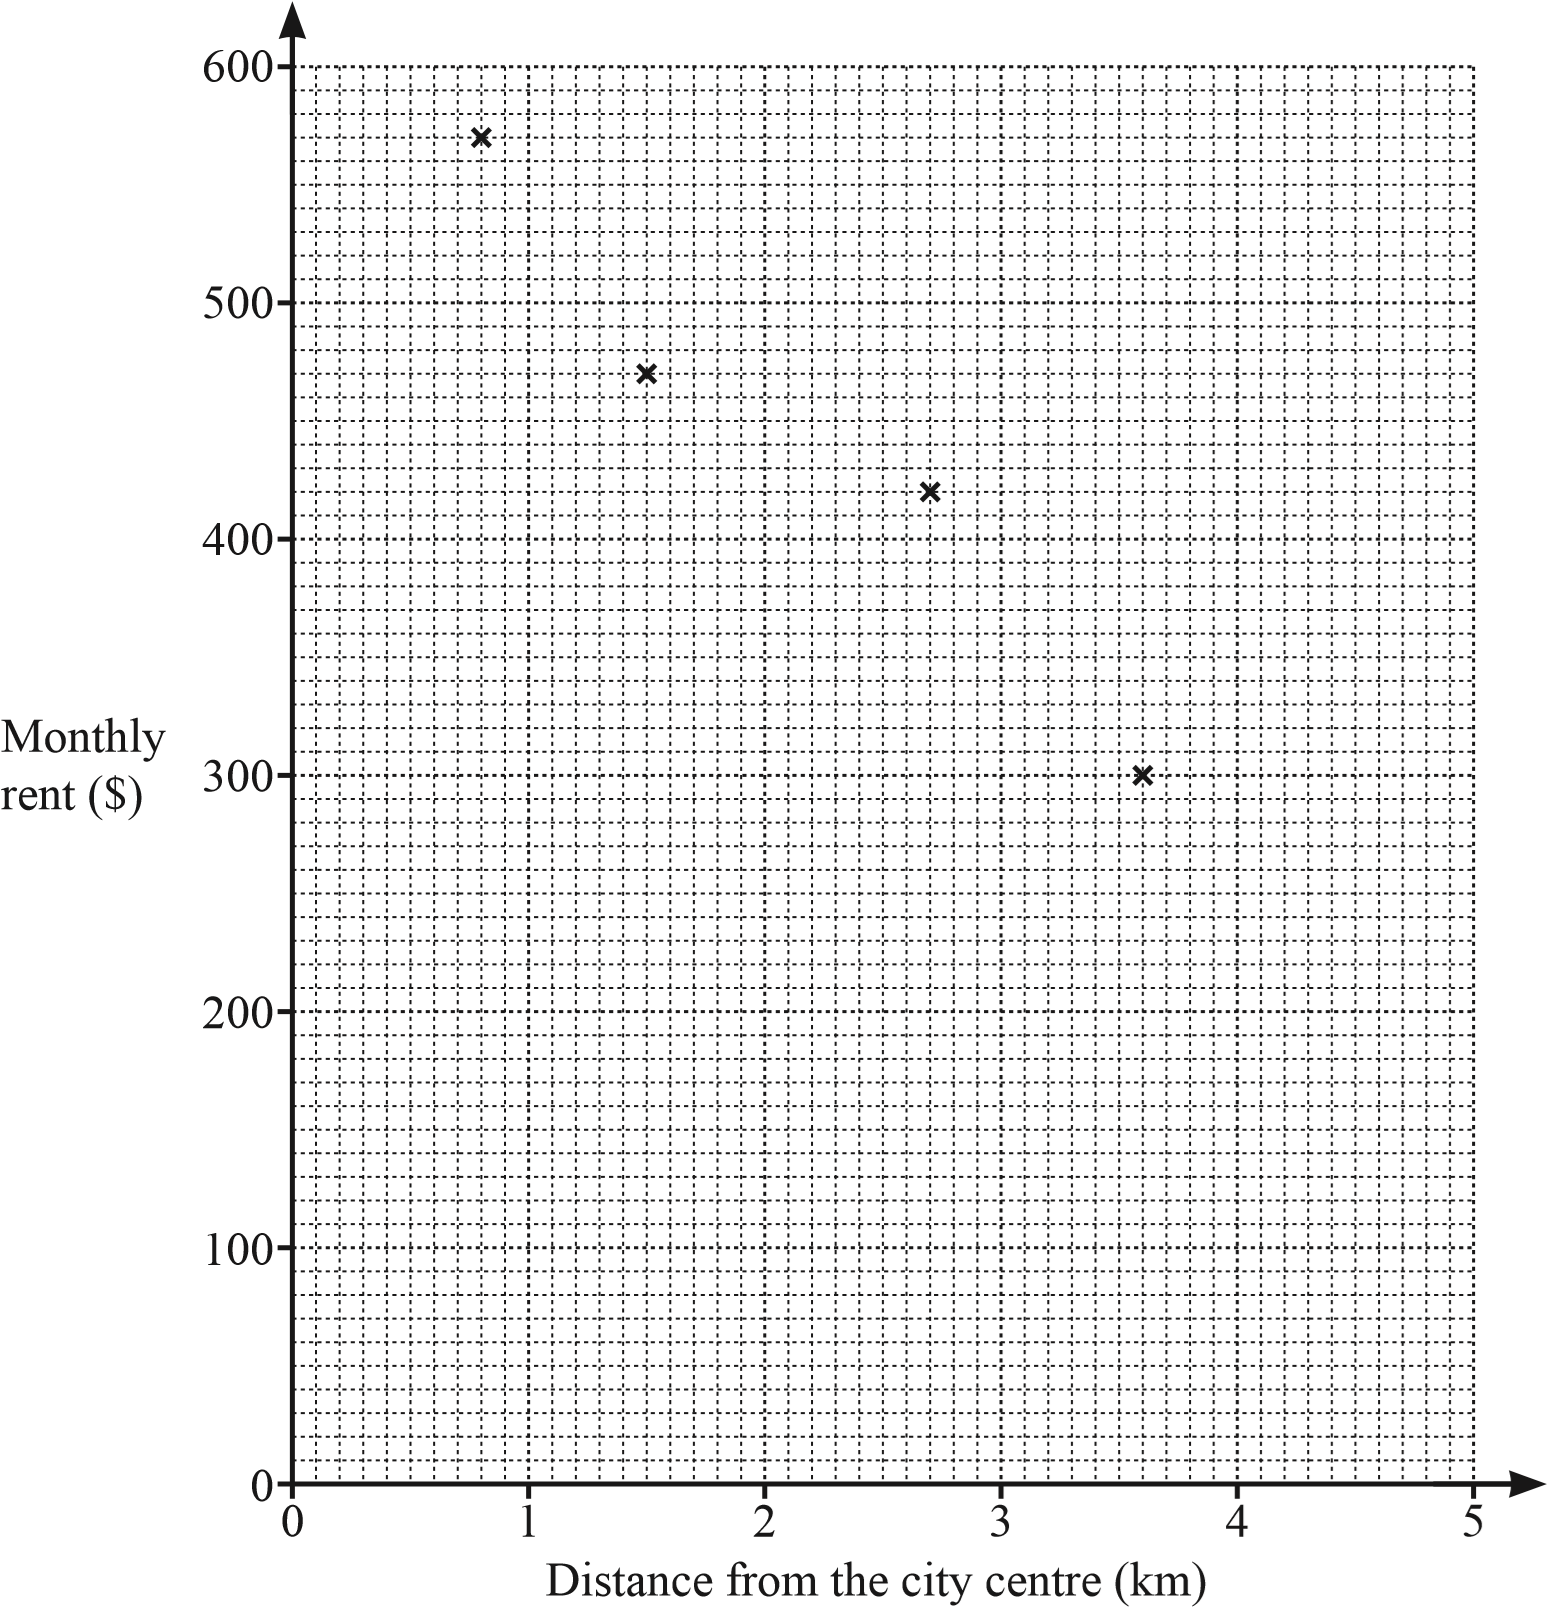
\includegraphics[scale=1]{Questions/quiz 10/images/Picture3.png}
\end{center}
\begin{parts}
\part 
Complete the scatter diagram.\\
 The first four points have been plotted for you.\\
{\flushright{
\hfill          [2]}}
\\ \\
\part What type of correlation is shown on the scatter diagram?\\
{\flushright{
\hfill          \makebox[12em]{\dotfill}  [1]}}\\
\part On the scatter diagram, draw a line of best fit.\quad \quad \quad \quad \quad \quad \quad \quad \quad \quad \quad \quad \quad \quad \quad \quad \quad
         [1]\\ 
\part Use your line of best fit to estimate the monthly rent for an apartment which is 4 km from the city
centre.\\ 
{\flushright{
\hfill          \$\makebox[12em]{\dotfill}  [1]}}\\
\end{parts}